% !TEX root = ../main.tex
%
\chapter{Health Index Estimation}
\vspace*{-15mm}\hfill{\fontfamily{phv}\normalsize\emph{Selami Hoxha and Gourav Prakash}}
\label{sec:hi_estimation}

\cleanchapterquote{Estimating is what you do when you don't know.}{Sherman Kent}{(Yale University professor)}

% \Blindtext[2][1]
This chapter introduces Health Index (HI) as an important tool for performing predictive maintenance. First, we
present the motivating factors for constructing a HI and its role in predictive maintenance in section \ref{sec:hi_estimation:motivation}.
The formal definition of the HI is given in section \ref{sec:hi_estimation:formal_definiton}. In section
\ref{sec:hi_estimation:datasets} there are presented three publicly available datasets that are used for training
and evaluating the approaches presented in section \ref{sec:hi_estimation:approaches}. Section
\ref{sec:hi_estimation:approaches} contains six different approaches in detail. The approaches are based on
current research on machine learning algorithms and techniques for performing predictive maintenance. The
presented approaches are General Regression Neural Network (GRNN), Artificial Neural Networks (ANN), Ensemble
methods, LSTM Encoder Decoder, Hierarchical Gated Recurrent Unit (HGRUN) and Kullback-Leibler Divergence. Finally,
in section \ref{sec:hi_estimation:evaluation} evaluation metrics are presented.


\section{Motivation}
\vspace*{-15mm}\hfill{\fontfamily{phv}\normalsize\emph{Gourav Prakash}}
\label{sec:hi_estimation:motivation}

The world is moving towards an era of technology where machine performance takes precedence over labor. There are
many drawbacks to this development, including a large amount of data and different types of machines that must be
updated to avoid certain bugs that can cause a huge loss of resources and financial support. Predictive maintenance
plays an important role in solving this problem. The predictive maintenance strategy can estimate the current state
of the system and predict the future state of the system. There are many techniques that can be used to predict
system operating conditions. One of these techniques is the Health Index (HI). It estimates the current state of
the system and monitors it over a period of time. The HI estimates the health of
the system by setting its state between 0 and 1, with a value closer to 1 indicating that the system is in good
condition, while a value closer to 0 indicates a system failure.

% Over the past few decades, the HI has become an increasingly 
% popular tool for predictive maintenance strategies. 
% Using the HI as an estimator can help estimate the state 
% of the system.where (i.e., 100\%) 
% means the system is in good health while 0 (i.e., 0\%) means system 
% failure. These values ​​can be shown graphically
% as a deterioration curve. By drawing these data over
% a specific timestamp, histories of the data
% collected can be created.

% \Blindtext[2][2]

\newpage
\section{Formal problem definition}\label{sec:Fpd_HI}
\vspace*{-15mm}
\hfill{\fontfamily{phv}\normalsize\emph{Gourav Prakash}}
\label{sec:hi_estimation:formal_definiton}

The health index is a state assessment index that acts as an approximation  of the current health of the system. The
health index of the system is a value that ranges between 0  and 1. A value close to 1 represent a healthy system,
and a value close to 0 indicates an unhealthy system or complete system failure.

The health index estimator $h$ maps the historical sensor data to health index values.  Formally, given data $x\in X$
we learn an estimator $ h : X \rightarrow Y $, which predicts the health index $y$ of a system. The input space $X$
contains of time series data as mentioned in section \ref{sec:intro:time-series-definition}. The output $y \in Y$ is
the estimated health index, where the output space $Y = [0,1] $.

To learn a health index estimator, we use training data from the set $D_{train}$ which contains $N$ instances of the
time series data denoted by $x_i$. The training data is of the form
\begin{equation}
    D_{train} = \{x_i\}_{i=1}^N.
\end{equation}
To evaluate the performance of the HI estimator, we use the test set
which has the form
\begin{equation}
    D_{test} = \{(x_i,y_i)\}_{i=1}^M ,
\end{equation}
where $y_i$ is the corresponding HI value for the instance
$x_i$.
% \\\\The performance of HI estimator for test data is measured using a loss
% function.
% \begin{equation}
%     \mathcal{L}(D_{test}) =\frac{1}{N} \Sigma_{i=1}^N 1-\sigma_i
% \end{equation}


% \Blindtext[3][2]

\newpage
\section{Publicly Available Datasets}
\vspace*{-15mm}
\hfill{\fontfamily{phv}\normalsize\emph{Selami Hoxha}}
\label{sec:hi_estimation:datasets}

In this section three datasets are presented. The milling dataset was created by performing lab experiments on
a milling machine \cite{millingData}. The bearing dataset was also created on a lab experiment where a motor
and a rotating shaft with four bearings was used \cite{bearingData}. The air quality dataset was created in a
field where different air quality factors were measured \cite{airQualityData}.

\subsection{Milling Dataset}
\label{sec:hi_estimation:datasets:milling_dataset}

The milling dataset \cite{millingData} is a created by performing lab experiments in a milling machine. The
experiments are run-to-failure experiments. The main purpose of the experiment is tool wear investigation. The
tool wear is measured under various operating conditions, where the conditions of the experiment are determined
by the fields DOC (depth of cut), feed (sideway cut), and type of material. Each of these fields has 2 settings,
which gives a total of 8 possible settings in which the machine was run. The depth of cut can be 1.5mm or
0.75mm; feed can be 0.5mm\textbackslash rev or 0.25mm\textbackslash rev (rev for revolution); the material is 1
for cast iron and 2 for steel. For each of the 8 settings the experiment was run 2 times, where each of the runs
is marked with a case number from 1 to 16, and is recorded in the field "case". In the experiment sensors for
measuring the current of the spindle, the vibration of spindle and table, and the acoustic emission of spindle and table
were setup. The dataset is organized in a ".mat" file and contains an array of 167 structs. Each struct contains
the 13 fields. The sensor measurements are recorded on arrays of type double with 9000 elements, and are recorded
in the fields smsAC, smsDC, vib\_table, vib\_spindle, AE\_table and AE\_spindle. Table
\ref{sec:hi_estimation:datasets:milling_table} shows all the fields and their description.

\begin{table}[ht]
    \centering
    \begin{tabular}{| l | l | }
        \hline
        \textbf{Field Name} & \textbf{Description}                        \\
        \hline
        case                & case number (1-16)                          \\
        \hline
        run                 & number of runs                              \\
        \hline
        VB                  & flank wear, was not measured after each run \\
        \hline
        time                & duration of experiment                      \\
        \hline
        DOC                 & depth of cut                                \\
        \hline
        feed                & feed                                        \\
        \hline
        material            & material                                    \\
        \hline
        smcAC               & AC current of spindle                       \\
        \hline
        smcDC               & DC current of spindle                       \\
        \hline
        vib\_table          & table vibration                             \\
        \hline
        vib\_spindle        & spindle vibration                           \\
        \hline
        AE\_table           & table acoustic emission                     \\
        \hline
        AE\_spindle         & spindle acoustic emission                   \\
        \hline
    \end{tabular}
    \vspace{0.3cm}
    \captionsetup{justification=centering}
    \caption{Fields and their description of milling dataset}
    \label{sec:hi_estimation:datasets:milling_table}
\end{table}




\subsection{Bearing Dataset}
\label{sec:hi_estimation:datasets:bearing_dataset}

The bearing dataset \cite{bearingData} consists of three datasets. Each dataset is collected from performing a
respective test-to-failure experiment. The experiments are performed in the same setup, but using different number
of sensors. The experiment is setup with a motor that rotates a shaft, and the shaft has four bearings. For
creating set 1 two accelerometers were used for each bearing, meanwhile for set 2 and 3 one accelerometer for each
bearing is used. In each experiment the data is collected every 10 minutes for 1 second with a frequency of 20kHz
(except for dataset 1 in which the first 48 recordings are done every 5 minutes). Every file consists of 20480 data
points which have eight columns for set 1 and four columns for set 2 and 3, which correspond with the number of
sensors in each experiment. The name of the file is the time step when the measurements are made. A summary of
these datasets is given in table \ref{sec:hi_estimation:datasets:bearing_table}.

\begin{table}[ht]
    \centering
    \renewcommand{\arraystretch}{2}
    \begin{tabular}{| l | l | l | l | }
        \hline
        \textbf{Set number} & \textbf{Columns} & \textbf{Number of files} & \textbf{Reason for failure} \\[0.2cm]
        \hline
        1                   & 8                & 2156                     &
        \parbox{6cm}{Bearing 3 had an inner race defect                                                 \\ Bearing 4 had a roller element defect}       \\[0.2cm]
        \hline
        2                   & 4                & 984                      &
        Bearing 1 had an outer race failure                                                             \\
        \hline
        3                   & 4                & 6324                     &
        Bearing 3 had a outer race failure                                                              \\
        \hline
    \end{tabular}
    \vspace{0.3cm}
    \captionsetup{justification=centering}
    \caption{Bearing datasets short description}
    \label{sec:hi_estimation:datasets:bearing_table}
\end{table}


\subsection{Air Quality Dataset}
\label{sec:hi_estimation:datasets:air_quality_dataset}

Air quality dataset \cite{airQualityData} authored by Saviero De Vito was developed in a 13 month period which resulted in
9358 instances. The data was gathered in a field in a polluted area in Italy. The device used for measurements was made of a sensor
array, a data processing unit and communication unit.The sensor array is used to take measurements for 5 metal oxide chemicals.
The 5 chemicals are CO, Non-Metanic Hydrocarbons (NMHC), Benzene, Total Nitrogen Oxides (NOx) and Nitrogen. The data processing
unit was capable to save sensor data for up to 72 hours with a 8 seconds sample rate (one sample every 8 seconds). These saved
recordings were then averaged hourly to form the instances (every hour one instance was generated). Finally, the instances and
were communicated to a data sink using the communication unit. The experiment is described in detail in \cite{DEVITO2008750}.


\begin{table}[ht]
    \centering
    \begin{tabular}{| l | l | }
        \hline
        \textbf{Field Number} & \textbf{Description}                               \\
        \hline
        0                     & Date                                               \\[0.1cm]
        \hline
        1                     & Time                                               \\[0.1cm]
        \hline
        2                     & CO in $mg\backslash m^3$                           \\[0.1cm]
        \hline
        3                     & PT08.S1 (CO targeted)                              \\[0.1cm]
        \hline
        4                     & Non Metanic HydroCarbons in $micro\backslash gm^3$ \\[0.1cm]
        \hline
        5                     & Benzene in $microg\backslash m^3$                  \\[0.1cm]
        \hline
        6                     & PT08.S2 (NMHC targeted)                            \\[0.1cm]
        \hline
        7                     & NOx concentration in ppb                           \\[0.1cm]
        \hline
        8                     & PT08.S3 (NOx targeted)                             \\[0.1cm]
        \hline
        9                     & NO2 in $micro\backslash gm^3$                      \\[0.1cm]
        \hline
        10                    & PT08.S4 (NO2 targeted)                             \\[0.1cm]
        \hline
        11                    & PT08.S5 (O3 targeted)                              \\[0.1cm]
        \hline
        12                    & temperature in $^{\circ}C$                         \\[0.1cm]
        \hline
        13                    & Relative humidity in percentage                    \\[0.1cm]
        \hline
        14                    & Absolute humidity                                  \\[0.1cm]
        \hline
    \end{tabular}
    \vspace{0.3cm}
    \captionsetup{justification=centering}
    \caption{Features in the air quality dataset}
    \label{sec:hi_estimation:datasets:air_quality_table}
\end{table}

\newpage
% \Blindtext[4][2]
\section{Approaches}
\vspace*{-15mm}\hfill{\fontfamily{phv}\normalsize\emph{Selami Hoxha and Gourav Prakash}}
\label{sec:hi_estimation:approaches}

In this chapter we are presenting six different state of the art approaches for estimating a HI. The title of each section
represent the machine learning method that was used to create the model. The approaches presented are: section \ref{sec:hi_estimation:approaches:GRNN}
General Regression Neural Network (GRNN), section \ref{sec:hi_estimation:approaches:hi_based_rul} Artificial Neural Network (ANN),
section \ref{sec:hi_estimation:approaches:ensemble_technique} Ensemble Learning, section \ref{sec:hi_estimation:approaches:lstmencoder}
Long Short-Term Memory - Encoder Decoder (LSTM-ED), section \ref{sec:hi_estimation:approaches:HGRUN} Hierarchical Gated Recurrent Unit Network (HGRUN), and
section \ref{sec:hi_estimation:approaches:kullbackLeibler} Kullback-Leibler Divergence (KLD).


% \Blindtext[2][1]
\subsection{General Regression Neural Network (GRNN)}
\vspace*{-18mm}\hfill{\fontfamily{phv}\normalsize\emph{Gourav Prakash}}
\label{sec:hi_estimation:approaches:GRNN}

The General Neural Regression Network (GRNN) is a radical-based neural network. It can be used to calculate health
Index (HI) of the system or subsystem. Its interpolation and quick adaptation properties for learning the dimension
Mapping very quickly makes it a popular technique in estimating the system's HI. Generally GRNN
Parameters can be derived directly from the finite set of training measurements. As stated in paper
\cite{Islam2018CalculatingAH}, $Y=Y_n$ as an dependent variable is predicted using a $D$-dimensional number of independent
input $X=X_n$, $X_n\in R^D$, where $D$ is a number of tests conducted on the system and $R$ is the quantitation level
of every measurements.


The mapping structure for GRNN $G(x)$ is to map the input $X$ to the output $Y$ based on finite set of $n$
measurements, where either space can be multi-dimensional. The basic equation for GRNN function G(x) based on Gaussian
kernel \cite{Vert2004APO} can be written as:

\begin{equation} \label{Equation_1}
    G(x)=\frac{\Sigma_{n=1}^N Y_n K(x,X_n)}{\Sigma_{n=1}^N K(x,X_n)}
\end{equation}
where:
\begin{itemize}
    \item $Y_n$ is the HI score for training set $X_n$.
    \item $K(x,X_n)$ is the Gaussian kernel.
\end{itemize}
\paragraph{Gaussian Kernel:}
\begin{itemize}
    \item $K(x,X_n)=e^(\frac{{-D_n}^2}{2})$,
    \item $D_n = (x-X_n)^T \Sigma^{-1} (x-X_n)$.
\end{itemize}
 
Where, $D_n$ is the distance between the training set $X_n$ and the point of prediction $x$. $\Sigma$ is multivariate
standard deviation.

The most common challenge in this approach is to find the optimal value of $\Sigma$ for the training set which
is known as smoothing parameter. If the value of $\Sigma$ increases then smoothens the model and some training
sample features are ignored while decreased $\Sigma$ values makes the model to overfits the training sample. This
overfitting makes the model case sensitive  and damages its generalization capability \cite{Islam2018CalculatingAH}.
The solution for this challenge is holdout methods. In this method, one sample is removed at a time from the training
set and the network is constructed from all other samples.

To collect the measurement from each subsystem, each measurement categories into four quantization levels with upper
and lower limits. These quantization level are considered as a condition ranges which has a mid point. The independent
variable $X_n=4^D$ of a training  set is developed using mid points of the conditional range for each test. The dependent
variable $Y_n$ is calculated by setting mid points in a value such as 0.25, 0.50, 0.75 and 1.0 where, lower value
represent bad condition and higher represent the good condition of the subsystem. The final value of $Y_n$ is the average
of their position scores.



To show the working process of GRNN model, a Gaussian kernel is used for its simplicity and smoothing probability. As,
stated in above paragraph, each measurement are considered to create a four quantization level. These quantization levels
has a sharper boundaries which are very sensitive. Any slight change in values leads to complete different conditional
ranges values.
This quantization is a drawback for this approach. To overcome this problem, a continuous function
needs to develop using a interpolation techniques. By which, the midpoint of the higher and lower point of each limits
are assigned with conditional ranges in GRNN model.

\begin{figure}[ht]
    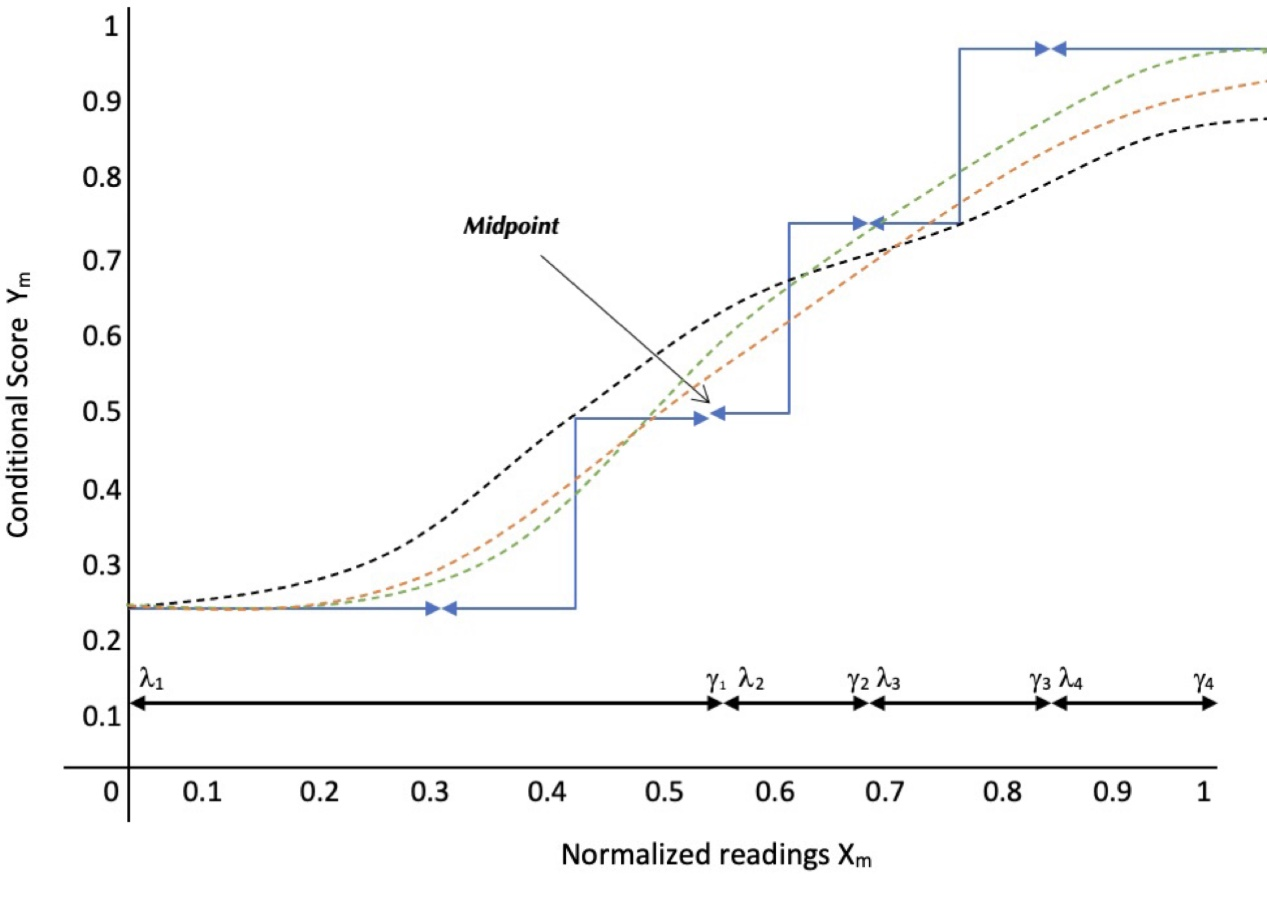
\includegraphics[width=\textwidth]{gfx/Quantizaton_Level.jpg}
    \captionsetup{justification=centering}
    \caption{GRNN interpolation of normalized and conditional.
        \cite{Islam2018CalculatingAH}.}
    \label{fig:Quant}
\end{figure}


The upper and lower limit can be represented in Figure \ref{fig:Quant} in $\lambda$ represents the lower limit and $\gamma$ represents the upper limit of four
conditional ranges.


Representation of four conditional ranges with upper and lower limits are as follows:
\begin{center}
    $Limit Values =
        \begin{bmatrix}
            \lambda_1,D & \lambda_1,D \\
            \lambda_2,D & \lambda_2,D \\
            \lambda_3,D & \lambda_3,D \\
            \lambda_4,D & \lambda_4,D \\
        \end{bmatrix}$
\end{center}

where, $\lambda_i,D = \lambda_i+1,D$ for next ranges and so on. while the targeted midpoint for each quantization
region can be written as
\begin{equation}\label{Equation:4.4}
    \theta_m,D = \frac{\lambda_m,D + \gamma_m,D}{2},
\end{equation}
where $m$ is the quantization levels.

In this approach GRNN is stated as a step function. Due to interpolation technique small changes in measurement of
standard deviation $\Sigma$ does not effect much on the condition score near the boundaries which results in identical
score.

\subsubsection{Feature extraction for HI calculation}
The training set used for GRNN model is the $X_n=R^D$. To get $X_n$ values the mid points of four conditional limits
the conditional score  values(0.25, 0.50, 0.75 and1.0) are represent as Good, Fair, Poor and Very poor. To calculate
the HI score $Y_n$ for each combination of training set $X_n$, the average of each corresponding scores was taken. For
example, if two tests conducted on the subsystem and the test scores are the midpoint of Fair and Very poor, then the
HI score $Y_n$ will be the average of 0.75 and 0.25 which is 0.50. These, $X_n$ and $Y_n$ values are used to train the
GRNN model.

To smoothen the GRNN model, the holdout method is used to calculate the covariance $\Sigma$ stated in
equation \ref{Equation:4.4} for Gaussian Kernel. In holdout approach, one sample from every training set is removed simultaneously and
network is constructed using remaining samples. The network is used to estimate the HI score of a missing sample at a
small values of $E$. Where, $E$ is a multiplicative factor used to provide an appropriate amount of smoothing. The
holdout process is repeated for all sample and the mean- squared error is estimated and stored.

Then, the value of
multiplicative factors is increased in a straight line to 1 with a small incremental step and the whole process is
repeated. Then the mean square for all values of $E$ is plotted. These values used as a multiplicative factor for
$\Sigma_s$, where $\Sigma_s$ is covariance of $X_n$. The process ensure the optimal smoothing to GRNN interpolation for
each subsystem of training set $X_n$. Finally, using equation \ref{Equation_1} the HI score is calculated.


\subsection{Artificial Neural Networks (ANN)}
\vspace*{-12.5mm}\hfill{\fontfamily{phv}\normalsize\emph{Gourav Prakash}}
\label{sec:hi_estimation:approaches:hi_based_rul}

The use of data-driven approaches has gained more popularity due to its non-requirement of prior knowledge of physical
and analytical models with measured data, to predict the future degradation behavior of a system. Data-driven approaches
rely on historically collected data to derive models directly from the data for Remaining Useful Lifetime (RUL) prediction.
Based on this data-driven techniques the RUL can be predicted using HI. In HI-based RUL prediction the model for input
signals against HI is build first and then mapped to estimated HI for RUL.

\subsubsection{HI degradation}

HI estimates the the system health. The heath index is mapped on a graph in respect to time as a degradation line. This
degradation graph represent the the system health index over certain time period. The degradation of HI can be linear or
non-linear. Linear and non-linear graph degradation of HI Figure \ref{fig:HI_Degradation}.

\begin{figure}[ht]
    \centering
    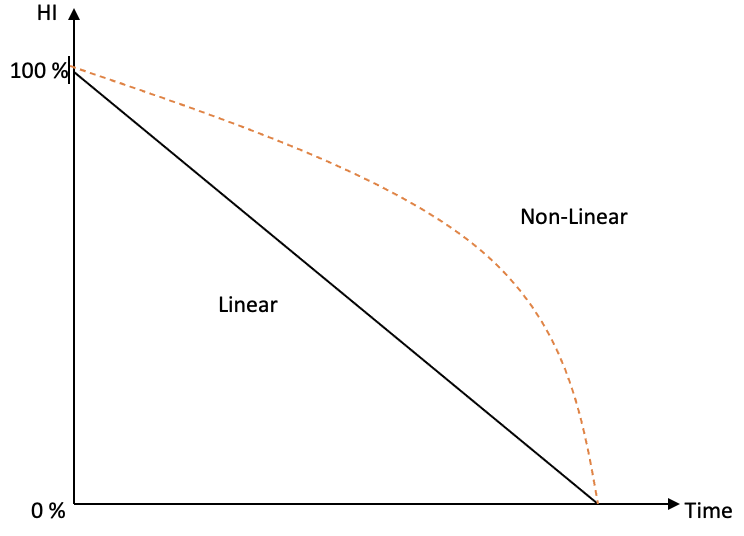
\includegraphics[width=\textwidth]{gfx/HI_Degradation}
    \captionsetup{justification=centering}
    \caption{Linear and non-linear degradation of HI}
    \label{fig:HI_Degradation}
\end{figure}


HI degradation can be linear or non-linear. Linear HI degradation is best known for its simplicity and its easy to
implement. While, non-linear HI degradation is complicated and requires prior knowledge of the system degradation pattern.

\paragraph{Modeling algorithm:}
HI-based RUL prediction is determined by the modeling algorithm. These
modeling algorithm has two stages. First stage is used to learn and predict the HI from instance and second stage is
used to get the RUL from HI. There are many existing modeling algorithm but this paper includes the linear and non-linear
regression model.

Both linear and non-linear models describes the relationship of HI to the time $t$. In case, where HI is shows as non-linear
degradation, a relationship function $f(.)$ is then build by learning algorithm (Neural Network) which makes
\cite{DBLP:journals/tie/YangHZXLN16}
\begin{equation}
    nonlinear[HI]=f(x).
\end{equation}
Similarly, for linear HI a mapping function $g(.)$ is used. By which its assumed that $linear[HI] = g(nonlinear[HI])$, because
Both linear and non-linear model have same ranges between 0,1 and its shows the HI degradation over time $t$. Therefore,
\begin{equation}
    linear[HI] = g(nonlinear[HI]) = g(f(x)) = h(x)
\end{equation}
where, h(.) is the learning algorithm.

\subsubsection{Data Normalization}
Based on the linear degradation HI, data from each of the training motors are used to build multiple independent Neural network
models for predicting HI's. After dynamic smoothing process the HI's are then mapped to the predicted RUL's upon which the
predicted RUL's are assembled to get the final RUL prediction.

During the HI prediction, each testing instance is then normalized based on the parameters calculated from the training instances.
z-score approach
\begin{equation}
    z=\frac{x-\mu}{\sigma}
\end{equation}

where, $\mu$ and $\sigma$ are the mean and standard deviation of a feature in the training data, $x$ is original data, and $z$ is
the normalized data of the features.

\subsection{Ensemble technique}
\vspace*{-12.5mm}\hfill{\fontfamily{phv}\normalsize\emph{Gourav Prakash}}
\label{sec:hi_estimation:approaches:ensemble_technique}

There are several prognostic approaches that are being used to predict the RUL for complex system. One of those prognostic approaches
Ensemble technique is most popular and reliable because of its increase in accuracy and robust behavior. The ensemble predictive
model uses the different ML algorithms or models that are developed using the almost identical datasets which results gives a better
performance compared to single modeling techniques.

The prognostic methods rather than physical and hybrid based it can also be defined as data-driven approach. In data-driven approach
we take the historically collected data and derive the models directly from those data fro the RUL prediction, instead of failure
mechanisms. Data-driven  techniques, the approaches are divided into into categories. FIrst, Direct RUL estimation that models the
relationship between input signals and RUL. Second, HI-based prediction, that uses HI as the training target then map the HI on the RUL.

In this approach we are going to see the HI based techniques to predict the RUL using Ensemble methods. Ensemble methods construct a set
of hypotheses and combine them together. This strengthen the learning algorithm and increase the accuracy of the prediction.

\subsubsection{Methodology}

To develop a predictive model for HI prediction, the raw data were used to extract the valuable information for training purpose regardless of
faulty propagation. To develop a predictive model, the ML algorithm learns the relationship between the training data and the target HI.For the testing phase, testing dataset are provided as input to the predictive model. Thus, the predictive HI is mapped to RUL as
illustrated in Figure \ref{fig:mipet}.

\begin{figure}[ht]
    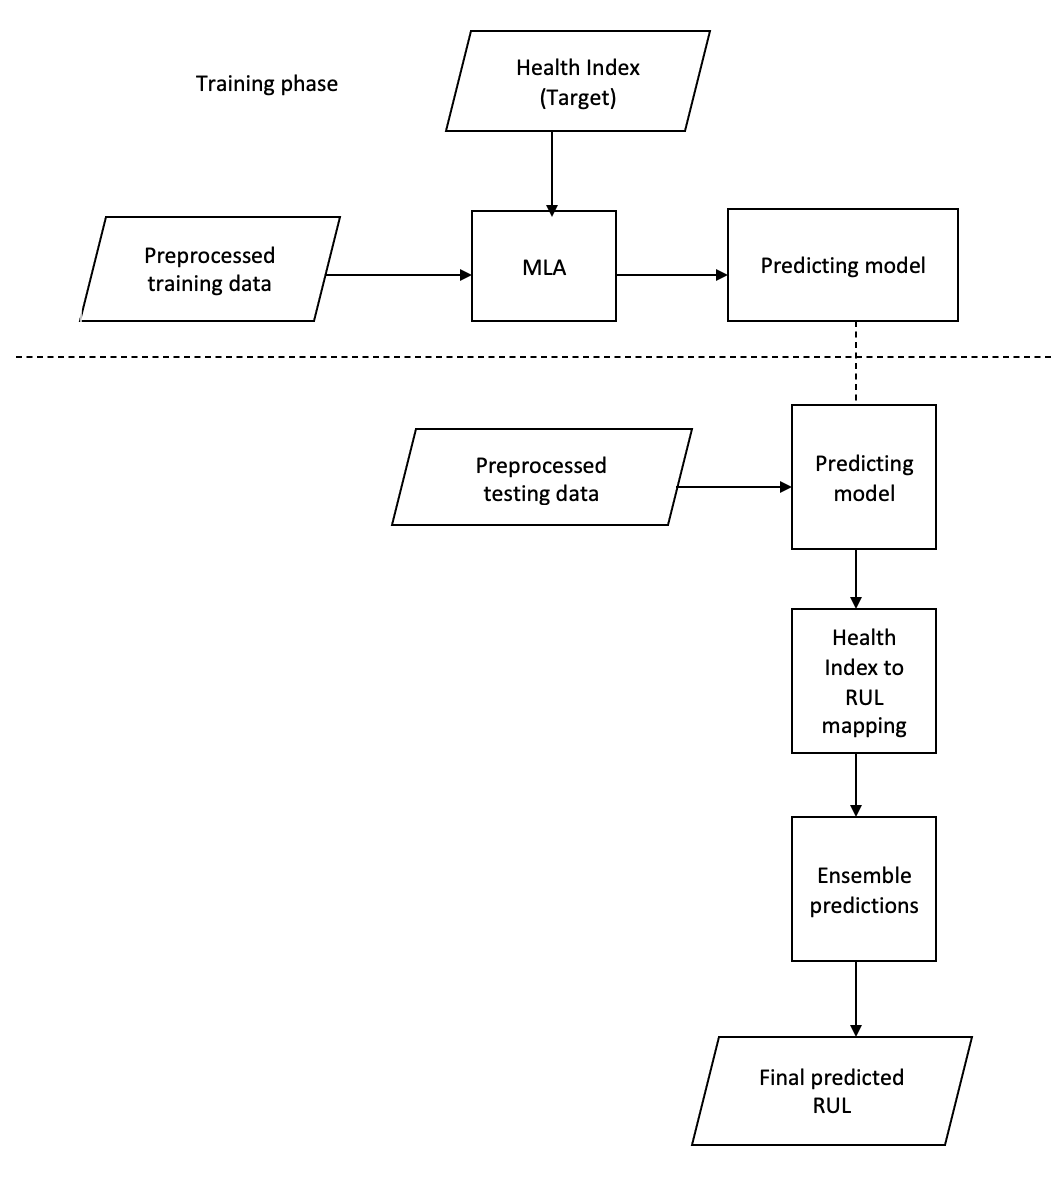
\includegraphics[width=\textwidth,]{gfx/mipet.png}
    \captionsetup{justification=centering}
    \caption{Methodology implementation phases
        \cite{Mutunga2019HealthIndexBP}.}
    \label{fig:mipet}
\end{figure}

\subsubsection{Data processing}
The data type used for this approach is the multi-variant time series data. Each training sample or unit was run to its failure at certain
time. The sensor collects the different measurements related to the system state at runtime.

\begin{figure}[ht]
    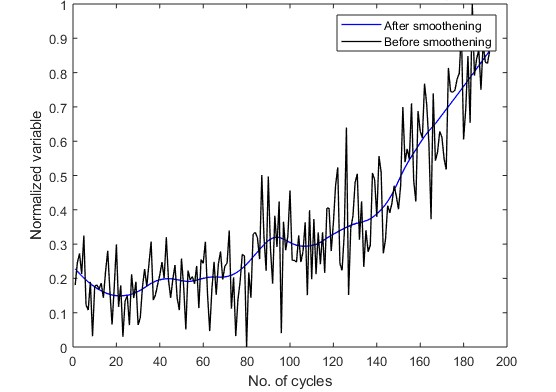
\includegraphics[width=\textwidth]{gfx/Nrmd.png}
    \captionsetup{justification=centering}
    \caption{Data smoothing effects.
        \cite{Mutunga2019HealthIndexBP}.}
    \label{fig:Nrmd}
\end{figure}

In order to identify a smaller subset from the main feature set, a feature selection process was carried out. To reduce the low monotonic values
a monotonicity function $M$ is used,
\begin{equation}
    M=\frac{no.of \frac{dx}{dt}>0-no.of\frac{dx}{dt}<0}{n-1}
\end{equation}

where,
$n$ is the number of observations in a feature, and $dx/dt$ is the derivative of the feature variables with respect to the cycles
\cite{Mutunga2019HealthIndexBP}. THe value of the $M$ ranges between 0 and 1 where, 1 represent the higher monotonic features and 0 represents
non-monotonic features. Therefore, the time variable together with sensors were used as a training datasets. Figure \ref{fig:Nrmd} shows effect of
data smoothing process to remove noises from the data thats allows the important pattern to be revealed. During data modeling, the normalization
$z$-score treats the outliers well, increasing their consistency, and making mapping inputs to the target more efficient.

\begin{equation}
    z=\frac{x-\mu}{\sigma}
\end{equation}

where,

$x$ is the dataset before normalization, $\mu$ and $\sigma$ are the mean and standard deviation for the corresponding variable respectively, and
$z$ is the normalized dataset.

\subsubsection{Auto-Regressive modeling}

Auto-Regression modeling(AR) map the predicted HI to the RUL.To predict the HI values to obtain the degradation trend a sequential representation
of model is illustrated by
\begin{equation}
    HI=\Sigma_{k=1}^m a_k x_{i-k}+e, i=1,2,3,...,n
\end{equation}
where, $a_k$ are the model parameters, $m$ is the model orders, $e_i$ is the model residual and $n$ no.of data points in HI.

\begin{figure}[ht]
    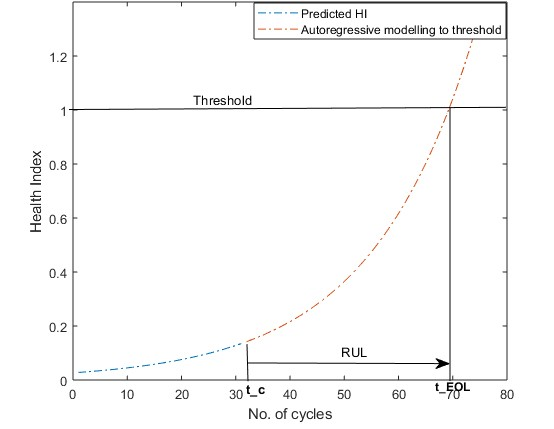
\includegraphics[width=\textwidth]{gfx/Autorm.png}
    \captionsetup{justification=centering}
    \caption{Auto-regression modeling.
        \cite{Mutunga2019HealthIndexBP}.}
    \label{fig:Autorm}
\end{figure}

Figure \ref{fig:Autorm} represents the predicted HI, which has the second section being the corresponding extrapolation to the set threshold of value 1
\cite{Mutunga2019HealthIndexBP}. Where, RUL is defined as the different in number of cycles between current time $t_c$ and the time at end of life
of the system $t_{EOL}$

\subsubsection{Ensemble Techniques}

In ensemble, for different ML algorithm similar datasets with various wearing condition is implemented first. For training datasets, the every similar
number of units the similar amount of predictive models are developed using ML algorithm. During the testing phase, test data for each unit are used as
input to each of the developed models and to the ensembled output. Then, the average are used to obtain the final RUL prediction. Based on the different
ML algorithm used as weighted averaging to aggregate the outputs \cite{Mutunga2019HealthIndexBP},
\begin{equation}
    RUL=\frac{\Sigma_{i=1}^n w_i RUL_i}{\Sigma_{i-1}^n w_i}
\end{equation}

where, $RUL_i$ is the RUL estimated by method $i,w_i$(assigned weight to method $i$ and $n$)which is the number of ML algorithm. For performance evaluation
the prognostics metrics which are selected for performance evaluation of the develop model were Mean Absolute Error($MAE$) , Mean Squared Error($MSE$) and
the Score function as stated in \cite{Mutunga2019HealthIndexBP}.

% For $MAE$ the error is defined as the different between the actual time to failure($AT$) and Estimated time to failure($ET$). So, Error according to $MAE$ is
% \begin{equation}
%     E=AT-ET
% \end{equation}

% Absolute error will be,
% \begin{equation}
%     |E|=|AT-ET|
% \end{equation}

The $MAE$ can be calculated as the average of the absolute error$E$ for each $n$ number of units.

% \begin{equation}
%     MAE=\frac{1}{n}\Sigma_{i=1}^n |E|
% \end{equation}

% Based on the $MAE$ the Mean Square Error $MSE$ is calculated as,
% \begin{equation}
%     MSE=\frac{1}{n}\Sigma_{i=1}^n E^2
% \end{equation}

The score function is the weighted sum of RUL errors and estimated metric score.

\begin{equation}
    S=s_1+s_2
\end{equation}

\begin{equation}
    s_1(E<0)=\Sigma_{i=1}^n e^{-\frac{E}{a_1}}
\end{equation}

\begin{equation}
    s_2(E\geq0)=\Sigma_{i=1}^n e^{\frac{E}{a_2}}
\end{equation}

where,
$S$ is the computed score, $n$ is the number of prediction units, and $E$ is the error terms.


\subsection{LSTM Encoder-Decoder}
\vspace*{-12.5mm}\hfill{\fontfamily{phv}\normalsize\emph{Selami Hoxha}}
\label{sec:hi_estimation:approaches:lstmencoder}

In the paper by Malhotra et al.,\cite{DBLP:journals/corr/MalhotraTRAVAS16}, an approach for estimating HI based on encoder-decoder
with hidden units being Long Short Term Memory (LSTM) units is presented and is called LSTM-ED (Long Short-Term Memory - Encoder Decoder).
A traditional way of calculating RUL for a system is to build a HI based on assumption that it follows a linear or exponential degradation
curve, where this curve is later extrapolated to a RUL. The problem with this approach is that the degradation of a system will not always follow
such a curve. LSTM-ED does not assume the shape of degradation curve. LSTM-ED will learn an
encoder-decoder model, then the model will learn an encoding of a sequence into some shorter representation and at the same time learns
to decode that encoded sequence into the original sequence. When this model is used for reconstructing to the original sequence, it will generate
some error which is called reconstruction error and is the basis of how the HI curve will be calculated.


\paragraph{Principal Component Analysis}
Principal Component Analysis (PCA) is an important tool which will be
used in a few approaches in this chapter, starting with LSTM-ED.
PCA is a dimensionality reduction algorithm. The dimensionality is reduced by projecting the data into a lower linear subspace
that minimizes the reconstruction error. Given the data matrix $X$, with N dimensions, where each element is centered to the mean of
the data, the PCA algorithm tries to find the optimal orthogonal projection matrix $P^{*}$ to the $k^{th}$ dimension by minimizing:
\begin{equation}
    P^{*} = \min_{P \in P_k} ||PX-X||_F^2
\end{equation}
where $P_k$ is the set of matrices that are N-dimensional and have a rank of $k$.
This way the dimensionality of X is reduced from N to k where $N>k$ without losing too much information
about the data. Another interpretation is that the dimensions with the biggest variance are kept. These k
dimensions that retain the most information about the data are called the principal components. \cite{MohriFML}

\paragraph{LSTM unit}
A LSTM unit or cell, is a neural network cell which is capable to process sequential data. It is structured in such a way that is able to
save important information about the input and forget the information that is not useful. The LSTM cell is made of several gates as shown
in figure \ref{fig:lstm_unit}. The gates process the data using the equations:
\begin{equation}
    \begin{aligned}
        i_t = \sigma(W_i h_{t-1} + W_i h_t)                          \\
        f_t = \sigma(W_f h_{t-1} + W_f h_t)                          \\
        o_t = \sigma(W_o h_{t-1} + W_o h_t)                          \\
        \tilde{c} = \tanh(W_{\tilde{c}} h_{t-1} + W_{\tilde{c}} h_t) \\
    \end{aligned}
\end{equation}

where $x_t$ is the input vector, $h_t$ is the output vector, $i_t$ is the input gate, $f_t$ is the
forget gate, $o_t$ is the output gate, $\tilde{c}$ is the intermediate memory cell, and W are the model
parameters.
Then the cell memory and the output vector are calculated and are both output to be processed
by the next cell. The cell memory and output vector are calculated by the following:
\begin{equation}
    \begin{aligned}
        c_t = (i_t  \tilde{c}_t) + (f_t c_{t-1}) \\
        h_t = o_t \tanh(c_t)
    \end{aligned}
\end{equation}
here $c_t$ is the cell state.
\cite{LSTMandGRU}

\begin{figure}[ht]
    \centering
    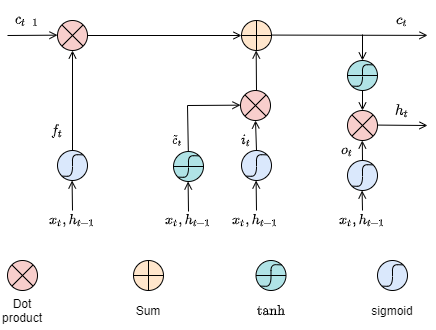
\includegraphics[scale=0.7]{gfx/LSTM_unit}
    \captionsetup{justification=centering}
    \caption{LSTM unit structure \cite{LSTMandGRU}}
    \label{fig:lstm_unit}
\end{figure}

\paragraph{HI construction}
Let us denote with $X^{(i)} = [x_i^{(1)} ,  x_i^{(2)} , \dots , x_{i}^{(\tau(i))}]$ with $x_i^{(t)} \in \mathbb{R}^{|S|}$ defined as in section
\ref{sec:intro:time-series-definition}
and $\tau(i) = \tau(i,s)$ for all $s \in S$ denotes the number of time steps until the end of life (the failure occurs) of
a system, which in this case is the assumed
to be the same for all the sensors. Next, the sensor data of each time step is z-normalized.
Let $\mu_j$ and $\sigma_j$ be the mean and standard deviation calculated sensor wise with j denoting the sensor. The
elements in  $X^{(i)}$ will take the form $\frac{x^{(t)}_{ij}-\mu_j}{\sigma_j}$, where $x^{(t)}_{ij}$ is the reading of $j^{th}$ sensor
of instance $i$ at time step $t$. Since in real world the sensor data is correlated, a
dimensionality reduction algorithm is applied. In our case PCA is applied to achieve what is called "the derived data" on
which the next steps will be taken. The derived data is denoted as $Z^{(i)} = [z_i^{(1)}, \,  z_i^{(2)}, \, \dots \, ,z_{i}^{(\tau(i))}]$ where
$z_i^{(t)} \in \mathbb{R}^p$, with $p$ being the number of principal components.

To train a LSTM ED network, subsequences of length \emph{l} from all the training instances are used. More precisely the first \emph{l} elements which
are assumed to represent a healthy state of the system are used for training.
First, the encoder is trained, given the time series
$Z = [z_1, \,  z_2, \, \dots ,z_l]$, $a_t^{(E)}$, the hidden state of the encoder at time $t$ for each $t \in \{1,2,\dots,l\}$, where
$a_t^{(E)}\in R^c$, with $c$ being the number of LSTM units in the hidden layer of the encoder. The decoder is trained jointly with
the encoder. The decoder is initialized in the reverse order, hence the reconstructed time series is output in the reverse order $Z = [z_l, \,  z_{l-1}, \, \dots ,z_1]$. The process is shown in figure \ref{fig:LSTM_inference}.

\begin{figure}[ht]
    \centering
    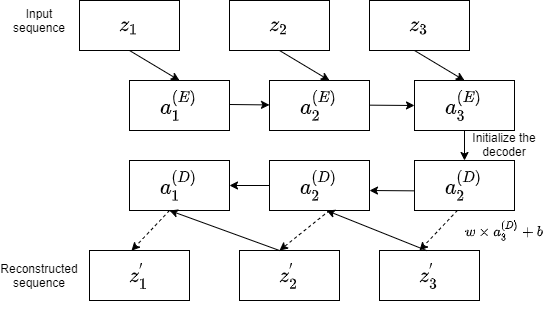
\includegraphics[scale=0.6]{gfx/LSTM_ED_inference}
    \captionsetup{justification=centering}
    \caption{LSTM-ED neural network structure
        \cite{DBLP:journals/corr/MalhotraTRAVAS16}}
    \label{fig:LSTM_inference}
\end{figure}

To reconstruct all the possible subsequences, a sliding window of size \emph{l} is used.
This means that there will
be $L-l+1$ subsequences of length \emph{l}. Also, it is important to note that an element $z_t$ will be calculated at most \emph{l} times,
or every time it is part of some subsequence. To get the final values an averaging is performed. Finally, the
reconstruction error for time step t is given $e_t^{(i)} = ||z_t^{(i)} - z_t^{'(i)}||$, where $z^{'}$ is the reconstructed sequence.
The model's optimization goal is to minimize
$E = \sum_{i\in[N]}\sum_{t=1}^{l}{{\left( e_t^{(i)} \right)}^2}$.

After the reconstruction error is calculated, it is scaled to obtain the target HI $h_t^{(i)}$ as:
\begin{equation}
    h_t^{(i)} = \frac{e_M^{(i)}-e_t^{(i)}}{e_M^{(i)}-e_m^{(i)}}
\end{equation} where $e_M^{(i)}$ and $e_m^{(i)}$ are the maximum and the minimum value of the reconstruction error respectively.

From the target HI calculated for each time-step $t$, we obtain a sequence of these HI which we call
the degradation curve. We note it by $H = [h^1_{(i)}, \, h^2_{(i)}, \, \dots ,\, h^{\tau(i)}_{(i)}]$.
For calculating RUL of the some new instance $i^*$, at first we need to build its degradation curve. The degradation curve is calculated
by first training a linear regression model for the time series data, where the target is the constructed HI. The Linear
regression has the form:

\begin{equation}
    f_{\theta}(z_t^{(i)})  = \theta^T z_t^{(i)} + \theta_0
\end{equation} where $\theta \in \mathbb{R}^p$, $\theta_0 \in \mathbb{R}$.



\subsection{Hierarchical Gated Recurrent Unit Network}
\vspace*{-12.5mm}\hfill{\fontfamily{phv}\normalsize\emph{Selami Hoxha}}
\label{sec:hi_estimation:approaches:HGRUN}

Gated Recurrent Unit Network (GRUN) is a Recurrent Neural Network (RNN) that has been successfully applied in health prognosis. In the paper
by Li et al., \cite{LI2019229},
the GRUN approach is used to determine HI degradation based on bearing historical data, which is used to determine future HI and
calculate RUL of the bearings. The approach presented in the paper is described in detail in the following.\\

\paragraph{Gated Recurrent Unit}
A gated recurrent unit is a variant of LSTM unit with a simplified architecture. It is made of an update gate which determines how
the hidden state $h_t$ will be modified by the candidate state $c_t$, and a reset gate which determines which part of the previous hidden
state $h_{t-1}$ to be ignored. The weights of GRU unit are calculated with a forward pass as follows:
\begin{equation}
    \begin{aligned}
        z_t = \sigma(W_{xz}x_t+U_{hz}h_{t-1}+b_z)             \\
        r_t = \tanh(W_{xr}x_t+U_{hr}h_{t-1}+b_r)              \\
        c_t = \tanh(W_{xc}x_t +U_{hc}(r_t \odot h_{t-1})+b_c) \\
        h_t = (1-z_t) \odot h_{t-1} + z_t \odot c_t
    \end{aligned}
\end{equation}
where $x_t$ is the input; $\sigma$ and $\tanh$ are the activation functions; $c_t$ is the candidate state; $h_t$ is the output of a unit;
$W_{xz}$, $W_{xr}$, and $W_{xc}$ are the weight matrices between the layers as noted in their subscript; $U_{hz}$, $U_{hr}$, and $U_{hc}$
are the weights of the cycles; $b_z$ $b_r$, and $b_h$ are the biases.

\begin{figure}[ht]
    \centering
    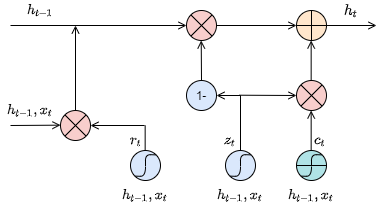
\includegraphics[scale=0.7]{gfx/GRU_unit}
    \captionsetup{justification=centering}
    \caption{GRU structure \cite{LSTMandGRU}}
    \label{fig:GRU_unit}
\end{figure}

\paragraph{The HI construction}

The HI is designed in several steps, starting with feature extraction, then applying a kernel principal component analysis (KPCA) to
extract the features that contain the most information about the data, followed by a smoothing via exponentially weighted moving
average (EWMA). The designed HIs are then used to learn a model using Hierarchical Gated Recurrent Unit Network (HGRUN)
which will be used to estimate HI for new instances of
time series data.
The first step in learning a model for the given time series data is to extract a set of features.
The process of feature extraction is given in detail in sections \ref{sec:feature-extraction:approaches:time-domain},
\ref{sec:feature-extraction:approaches:frequency-domain} and \ref{sec:feature-extraction:approaches:time-frequency-domain}.
The set of features is made of time domain, frequency domain and time-frequency domain features extracted from the time series data.
The features extracted from the time domain are Root mean square (RMS), absolute mean value (AE), square
root amplitude (SRA), variance and peak-to-peak value. From the frequency domain spectrum RMS, spectrum mean value and spectrum shape
factor are the extracted features. From time-frequency domain maximum value, RMS and SRA of the second-frequency-band signals, which are extracted
by the three-layer wavelet packet transformation. Only a handful of these high dimensional features will contain useful data. Therefore
the next step is to apply KPCA to extract the useful features. The KPCA performs PCA on data transformed to a higher dimensional feature space using
a kernel and then PCA is applied on the transformed data \cite{MohriFML}. The first step is to
map the data to a high dimensional space using the kernel and then applying the PCA algorithm to extract the actual principal components.
The first principal component $ p = [p_1,p_2,\dots,p_t]$ will be the HI, and will represent the bearing degradation. Since the HI
usually contains fluctuations, EMWA smoothing is applied. EMWA modifies the HI by approximating it with the value
\begin{equation}
    f_t = \alpha(p_t + \beta p_{t-1}+\beta^2p_{t-2}+\dots+\beta^{t-1}p_1).
\end{equation}
where $0< \alpha <1$ is called the smoothing parameter and $\beta$ is equal to $1-\alpha$. The value
$f_t$ is the HI after smoothing is applied and $p_t$ is the actual HI. The smoothed value is determined
by considering all the HI in the degradation curve, with the actual value $p_t$ having the biggest
influence and the other HI have exponentially decaying influence the farther they are in the degradation
curve.

\paragraph{The HGRUN model}

Since the rolling bearing degradation is is made of time-series parameters and since degradation is often nonlinear, a powerful
nonlinear model is required. To achieve such a powerful model, HGRUN is built with multiple GRU layers and with a regression layer
on top of the last GRU layer, as shown in fig \ref{fig:HGRUN_model}.

\begin{figure}[ht]
    \centering
    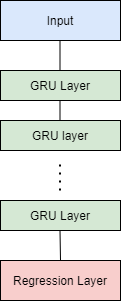
\includegraphics[scale=0.7]{gfx/HGRUN_model}
    \captionsetup{justification=centering}
    \caption{HGRUN structure}
    \label{fig:HGRUN_model}
\end{figure}

Since HGRUN is a RNN model, it is trained using back propagation through time and gradient descent.
The goal of the model is to minimize MSE.
\begin{equation}
    MSE = \frac{1}{2T}\sum_{t=1}^N (y_t-\hat{y}_t)^2
\end{equation}
where $y_t$ is the predicted value and $\hat{y}_t$ is the actual label. In the work presented AdaGrad
(Adaptive Gradient Descent) was used for fast convergence.
The AdaGrad algorithm is a modification of gradient descent and its parameters are updated
adaptively as follows:
\begin{equation}
    \begin{aligned}
        \eta_e = \frac{\eta_0}{\sqrt{\sum_{i=1}^e g_i^2 +\epsilon}} \\
        \upsilon_e = \mu \cdot \upsilon_{e-1} - \eta_e \cdot g_e    \\
        \theta_e = \theta_{e-1} + \upsilon_e
    \end{aligned}
\end{equation}
where $e$ is the epoch number; $\eta_e$ is the learning of the e-th epoch; $\epsilon$ is a value that ensures that the denominator
is never zero; $g_e$ is the e-th gradient; $\mu$ is the momentum; $\theta_e$ are the parameters at the e-th epoch and $v_e$ is the
e-th updating value.


\paragraph{Estimating the HI}

To predict future HI values a HGRUN model is also trained. The model is trained using training and testing samples which are designed
using the HI as calculated above. Suppose we have $N$ data points $(f_1, f_2, ... , f_N)$ calculated using the HI design explained
above for each time series raw samples. Using these N data points and the one-step look ahead technique, the samples for training and
testing HGRUN model are created. The first training example $e_1$ is formed by taking $(f_1, f_2, ..., f_{\emph{l}})$ as the sample
and $f_{\emph{l}+1}$ as the label. For the second example, the sample would be $(f_1, f_2, ..., f_{\emph{l}+1})$ and the label
$f_{\emph{l}+2}$. The training samples are formed until some point $k$, which means there are $N-l-k$ training samples. And then the
other data points $(f_k, ... , f_N)$ are used to create similarly the testing samples.

\subsection{Kullback Leibler Divergence}
\vspace*{-12.5mm}\hfill{\fontfamily{phv}\normalsize\emph{Selami Hoxha}}
\label{sec:hi_estimation:approaches:kullbackLeibler}

In the paper by Aremu et al.,\cite{DBLP:conf/indin/AremuOHM19} an approach based on information entropy is presented that captures the degradation of
multi sensor systems. PdM systems that perform condition monitoring based on raw data perform poorly according to the author.
An appropriate measure for the health condition of a system is needed to capture the degradation of the system accurately.
The multi sensor systems also pose a challenge for capturing the degradation of the system, since not all sensors have influence
on capturing the degradation of the system.  This is a model-free approach and is based on information entropy measure known as
Kullback-Leibler Divergence (KLD). As in LSTM-ED, it is assumed that the first \emph{l} time steps in the series
data represent a healthy state of a system. Then a tool that makes it possible to compare this representation
of the healthy system to other instances is used to build the HI.\\

The healthy state of the system in this work is represented by its distribution of the data. And in order
to compare the distribution of the entire
life of a system to the healthy data distribution the concept of entropy needs to be introduced. In
\cite{DBLP:conf/indin/AremuOHM19}, entropy is defined as:
'Entropy or information entropy is the measure of "unexpectedness" of data in a variable, obtained by quantifying its contained
uncertainty'. The entropy can be measured using the Shanon entropy, which is given by the formula:
\begin{equation}
    H(X) = - \sum_{x \in X} p(x) \log p(x)
\end{equation}
where $X$ is a random variable. The sum is over all the possible outcomes $x$ of the variable $X$ and
$p(x)$ is the probability of the distribution.
An important concept that is needed next is to be able to capture how much the distribution will change when some other event happens.
This change is measured by KLD. \newline Given the distributions $P$ and $Q$, KLD is given as follows:
\begin{equation}
    H(P||Q) := \sum_{x \in X} p(x) \log \frac{p(x)}{q(x)}
\end{equation}
with $H(P||P)=0$ and $H(P||Q) \neq H(Q||P)$ \\



Given the time series data $ X \in \mathbb{R}^{N \times u}$ where $N$ is the number of samples,
$u=|S|$ is the number of sensors and as before by $i$ we denote the $i^{th}$ instance of time series,
several steps are taken for the HI to be constructed. First, each sensor data
is used to parametrize a logistic distribution based on the first \emph{l} observations.

\begin{equation}
    X_i \sim \text{logistic}(\lambda_i, \sigma_i).
\end{equation}

The logistic distribution shape is determined by its parameters, with $\lambda$ being the location parameter that determines where the distribution will
be centered and $\sigma$ will determine how focused is the distribution around the center. A depiction of logistic distribution on two sets of parameters is
shown in figure \ref{fig:logistic_dist}.
Then, the probability density of each sensor data that represent a healthy system can be calculated by:
\begin{equation}
    f_i^s(x_i^s; \lambda_i^s, \sigma_i^s) = \frac{1}{\sigma_i^s}
    exp \bigg(-\frac{x_i^s - \lambda_i^s}{\sigma_i^s}\bigg){\bigg(1+exp \bigg(-\frac{x_i^s - \lambda_i^s}{\sigma_i^s}\bigg)\bigg)^{-2}}
\end{equation}

where we see that also the probability density function (pdf) is parametrized and $1<s<u$.

\begin{figure}[ht]
    \centering
    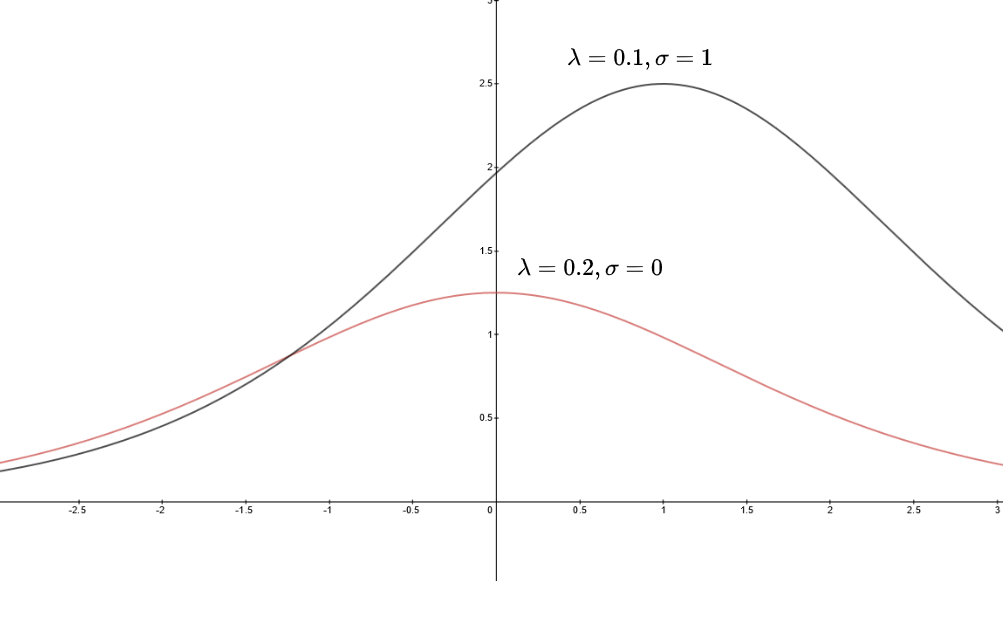
\includegraphics[scale =0.25]{gfx/logistic_dist}
    \captionsetup{justification=centering}
    \caption{Logistic distribution on two different sets of parameters}
    \label{fig:logistic_dist}
\end{figure}


Let $P^s$ be the distribution of observations in the healthy state of the system and $\zeta_k^s$ ($k=1,2,\dots, N$)
be the same distribution modified after seeing an observation from sensor s. The HI is defined as the KLD between the distributions $P^s$ and $\zeta_k^s$:
\begin{equation}
    H(P^s||\zeta_k^s) := \sum_{j=1}^{\emph{l}} \rho^s_j \log \frac{\rho_j}{\zeta_{kj}^s}
\end{equation}
where $1<k<N$.
\begin{equation}
    \rho_j^s = f_i^s(x_{i_j}^s; \lambda_i^s, \sigma_i^s)
\end{equation}
and
\begin{equation}
    \zeta_{kj} = f_i^s(y_j^s; \lambda_i^s=x_k^s, \sigma_i^s)
\end{equation}
where $y_j$ is generated by a random variable $Y^s$. $Y^s$ is a random variable generated by $X_n^s$ supported logistic regression with
the location parameter being the sample $x_k^s$. That means
\begin{equation}
    Y^s \sim \text{logistic}_{X_i^s}(\lambda_i = x_k^s, \sigma_i)
\end{equation}

Then the HI for a single sensor is given by:

\begin{equation}
    \hat{\emph{f}}_H^{\,\,s} = \{H(P^q||\zeta_1^s),H(P^q||\zeta_2^s),\dots ,H(P^s||\zeta_N^s)\}
\end{equation}


and finally the HIs of all the sensors are is given by the set:

\begin{equation}
    \label{sec:hi_estimation:kullback_leibler:HI_set}
    X_H = \big\{ \{ \hat{f}_H^{\,\, 1^T} , \hat{f}_H^{\,\, 2^T},\dots, \hat{f}_H^{\,\, u^T} \} \big\}
\end{equation}
.

If $H(P^q||\zeta_k^s) \neq H(P^q||\zeta_{k-1}^s)$ then wear has ocurred in the system.

\textbf{Selecting the sensors}

For performing feature selection, which in this case means selecting the sensors, KLD analysis of system complete lifecycle is evaluated.
This is done for each sensor using the following formula:
\begin{equation}
    \Delta_H^s =
    \left(H(P^q||\zeta_1^s)-H(P^q||\zeta_N^s)\right)
    \left(\frac{H(P^q||\zeta_1^s)+H(P^q||\zeta_N^s)}{2}\right)^{-1}
\end{equation}

If $\Delta_H^s$ is not greater than zero it means that the sensor does not show any degradation trend. Using this fact sensor selection
is performed by excluding the HI for the sensors that do not show any degradation trend. The set
of HI in equation \ref{sec:hi_estimation:kullback_leibler:HI_set} becomes:
\begin{equation}
    X_H = \big\{ \{ \hat{f}_H^{\,\, 1^T} , \hat{f}_H^{\,\, 2^T},\dots, \hat{f}_H^{\,\, u^T} \} | \Delta_H^s>0 \big\}
\end{equation}
.

Finally, the health indicator set can be used to train a supervised model where the target is the actual RUL.
This model can finally be used to estimate the RUL. Random forests and gaussian processes were applied in
the presented paper.

\newpage
\section{Evaluation}
\vspace*{-15mm}
\hfill{\fontfamily{phv}\normalsize\emph{Selami Hoxha}}
\label{sec:hi_estimation:evaluation}

The estimated HI should be a good representation of the actual state of the system for successful prognostics.
The evaluation of the HI is based on a test dataset, as presented in
\ref{sec:hi_estimation:formal_definiton}
which contains the instances of time series, that are not used
in the training process, and have information encoded for that instance. The information could be the actual
HI for every time step in the series, which is usually not the case in publicly available data, or the RUL. If we
have the actual HI for every time step in the test dataset, then using some metric we could compare the estimated value
with the actual value to measure its performance. Since publicly available datasets usually contain RUL, to get
the actual HI the RUL is extrapolated to an HI using some linear or exponential function
\cite{DBLP:journals/corr/MalhotraTRAVAS16} and this HI is compared to the estimated HI. Another way of measuring
the performance of HI is by using the estimated HI to get the RUL and then measure the performance by using some
metric that compares the actual RUL to the estimated one.

Several different metrics are being used in the research \cite{Islam2018CalculatingAH, LI2019229,
    DBLP:journals/tie/YangHZXLN16, Mutunga2019HealthIndexBP, DBLP:journals/corr/MalhotraTRAVAS16}. The metrics vary based on how
they handle late and early predictions.
A late prediction
is when the HI predicts that the system is healthier than it actually is, resulting in the system running into
failure before it can  be repaired. An early prediction is when the HI predicts
the system as lower than its actual value, which would mean that we repair the system that could have been functional for a longer time. The loss functions can be symmetric, where the late predictions and early predictions
are penalized equally, or asymmetric where the loss function has some parameter that decided on how to penalize
wrong predictions.
There are also metrics that operate on the whole degradation curve (represented by a vector of HIs ordered by the time step)\cite{DBLP:conf/indin/AremuOHM19}.

Let us denote by $y$ the actual value of HI or RUL, and by $\hat{y}$ the
estimated HI or RUL. Also, let $C$ denote the degradation curve. Finally, with $M$ is the
number of test instances.

\subsubsection{Symmetric loss functions}

Symmetric loss functions evaluate the estimated HI by penalizing the late predictions equally as early predictions. The smaller the loss, calculated using the loss functions,
the better the performance of the approach. In the following, symmetric loss
functions that are used for evaluating HI performance are presented.

\paragraph{Mean Squared Error}
\begin{equation}
    MSE = \frac{1}{M} \sum_{t=1}^M(y_t - \hat{y}_t)^2
\end{equation}
\cite{Islam2018CalculatingAH}.

\paragraph{Root Mean Squared Error (RMSE)}
\begin{equation}
    RMSE = \sqrt{\frac{1}{M-1} \sum_{t=1}^M(y_t - \hat{y}_t)^2}
\end{equation}
\cite{DBLP:journals/tie/YangHZXLN16}.

\paragraph{Maximum Absolute Error (maxAE)}
\begin{equation}
    maxAE = \max_{1 \leq t \leq M} (|y_t - \hat{y}_t|)
\end{equation}
\cite{LI2019229}.

\paragraph{Normal Mean Squared Error (NMSE)}
\begin{equation}
    NMSE = \frac{\sum_{t=1}^M (y_t - \hat{y}_t)^2}{\sum_{t=1}^M \hat{y}_t^2}
\end{equation}
\cite{LI2019229}.

\subsubsection{Assymetric score functions}

Asymmetric score functions evaluate an approach by penalizing early predictions and late
predictions in different amounts. Score functions are parametrized to achieve the
asymmetric evaluation. The bigger the score calculated by the score function
the better is the performance of the approach being evaluated.

\paragraph{Scoring function}

The scoring function can be used to penalize early predictions or late
predictions by controlling the parameters $\alpha_1$ and
$\alpha_2$.
\begin{equation}
    S=s_1+s_2
\end{equation}
where by denoting $E = y-\hat{y}$ we have, if $E<0$
\begin{equation}
    s_1 = \sum^M_{t=1} \exp{\left(-\frac{E}{\alpha_1}\right)}
\end{equation}
and if $E \geq 0$ then
\begin{equation}
    s_1 = \sum^M_{t=1} \exp{\left(\frac{E}{\alpha_2}\right)}.
\end{equation}
For both early and late predictions the error grows exponentially
\cite{Mutunga2019HealthIndexBP}.



\paragraph{Timeliness score}
Timeliness score is an asymmetric score function that is parametrized with the parameter $\gamma$,
where $\gamma = \frac{1}{a}$ if $\hat{y} - y \leq 0$ else $\gamma = \frac{1}{b} $ if $\hat{y} - y \geq 0$. If $a>b$ then late predictions ($\hat{y} - y \leq 0$) are penalized
more (by being divided with a greater number). Similarly, if $b>a$ then early prediction
will be penalized more.
This is formulated as follows:
\begin{equation}
    E = \sum_{i^* =1}^N (exp(\gamma |\hat{y} - y|)-1)
\end{equation}
Usually a > b is chosen, to
penalize late predictions more than early predictions \cite{DBLP:journals/corr/MalhotraTRAVAS16}.




\subsubsection{Degradation curve based evaluation functions}

A health degradation curve is the representation of the degradation of the health of the system.
The degradation curve is represented by HIs ordered in a sequence by the time step,
$C = [c_1, c_2, \dots ,c_K]$ with K
being the length of the sequence.


\paragraph{Monotonicity}
To evaluate if the HI degradation curve is a good representation of degradation of the system monotonicity measure and robustness measure are used. HI degradation curve should have an
increasing or decreasing degradation trend. Monotonicity is measured using the following metric:
\begin{equation}
    Mon(C) = \frac{1}{K-1}|N_{d/dc>0}-N_{d/dc<0}|
\end{equation}
where C is the HI degradation curve, the length of the HI curve is K and $d/dk=c_{k+1} - c_k$ is the difference between the HI in the sequence. The values range from 0 to 1,
where 1 indicates that the degradation curve is a good representation of the degradation
of the system (has strong monotonicity).
\cite{DBLP:conf/indin/AremuOHM19}.

\paragraph{Robustness}
Robustness measures the robustness of the HI degradation curve to noise. A good HI degradation
curve should be able to give good results in systems that
contain noisy data. The robustness measure is given by:
\begin{equation}
    Rob(C) = \frac{1}{K} \sum_{k=1}^K \exp \left(-\bigg| \frac{c_k-c_k^T}{c_k} \bigg|\right)
\end{equation}
where  $c_k^T$ is the mean value at $k^th$ element. The values range from 0 to 1, where
the value 1 represents a very smooth degradation curve.
\cite{DBLP:conf/indin/AremuOHM19}.